\documentclass[runningheads]{llncs}
\usepackage[T1]{fontenc}
\usepackage{graphicx}
\usepackage{amsmath}
\usepackage{amssymb}
%
%
\begin{document}
\title{Gated Scene-Specific YOLO: A Pruning and Gating Approach for Efficient Object Detection}
%
\author{Hector Acosta\inst{1}\orcidID{0009-0003-6784-8882} \and
Soon Ki Jung\inst{1}\orcidID{0000-0003-0239-6785}}
%
\authorrunning{H. Acosta et al.}
\institute{Kyungpook National University, Republic of Korea}
%
\maketitle              % typeset the header of the contribution
%
\begin{abstract}
In object detection, YOLO (You Only Look Once) has significantly advanced real-time applications. However, in dynamic environments, particularly on edge devices like security cameras, optimization is crucial. Our work introduces "Gated Scene-Specific YOLO," an adaptation of YOLO that includes a dynamic gating mechanism for improved efficiency. Traditional YOLO models often process excessive, irrelevant data. Our approach counters this by activating neural pathways relevant to the scene. This is achieved through dynamic gate generation during training and analyzing scenes to deactivate consistently inactive gates, streamlining the model for the environment's specific needs. This method reduces computational load while maintaining or improving detection accuracy, suitable for resource-constrained devices. Our results show that Gated Scene-Specific YOLO improves processing speed and maintains high accuracy, demonstrating the potential to enhance real-time object detection in various settings. This research contributes by showing a practical approach to optimize deep learning models for specific contexts, leading to more adaptable, resource-efficient detection solutions.
%
\keywords{Object Detection\and YOLO Architecture\and Scene-Specific Optimization\and Gated Neural Networks\and Model Pruning}
\end{abstract}
%
\section{Introduction}
Object detection is a cornerstone of computer vision, impacting a wide array of applications from surveillance to autonomous driving. The evolution of deep learning has propelled advancements in this domain, particularly through the YOLO (You Only Look Once) architecture by Redmon~\cite{redmon2016you}. Renowned for its efficiency in real-time processing, YOLO is a testament to the power of modern object detection systems from high-powered computing environments to more performance-constrained devices. While YOLO excels in real-time processing across these settings, its adaptability still faces challenges, especially when deployed on edge devices where computational resources are inherently limited. To address these challenges, our research specifically focuses on YOLOv6 by Li et al.~\cite{li2023yolov6,li2022yolov6}, known for its hardware-focused design and efficiency in real-time applications, forming an ideal base for our enhancements. In these scenarios, even the slightest optimization can yield significant improvements in speed and efficiency. Addressing this limitation, our research introduces "Gated Scene-Specific YOLO," a novel approach that integrates dynamic gating with scene-specific model pruning within the YOLO architecture.

In the world of neural network optimization, model pruning emerges as a promising solution to alleviate computational intensity. This technique focuses on trimming redundant or less significant parameters from a neural network, thus streamlining its structure with minimal impact on performance. Our methodology advances this concept by employing a dynamic gating mechanism that adapts to the unique features of the input scene, enhancing the object detection process's efficiency without compromising accuracy.

A key innovation in our approach is the use of Improved SemHash, a method initially introduced by Kaiser and Bengio~\cite{kaiser2018discrete} and further explored by Chen et al.~\cite{chen2019you}. This technique allows for the generation of binary gates during training, crucial for selectively activating or deactivating specific network filters in response to input variations. The process involves dynamically generating gates during training and then conducting an analysis phase for a specific scene. This analysis identifies gates that are consistently inactive and exports them for static application in real-world scenarios. As a result, the Gater Network, typically part of the backbone during training, can be excluded during actual deployment, relying instead on these statically determined gates for efficient and tailored object detection.

Our research introduces a significant advancement in the YOLO architecture through the integration of a gating network, intelligently deactivating filters based on the unique features of each input scene. This novel approach, enhanced by the incorporation of Improved SemHash~\cite{bengio2013deep,chen2019you}, not only allows for precise network activity control but also brings considerable improvements in computational efficiency and detection accuracy. Extensive experimental validation, focusing on metrics such as FLOPs, FPS, and mAP@0.5:0.95, demonstrates the efficacy of our strategy as we observed a significant increase in FPS compared to the YOLO counterpart of our pruned model, all without compromising the robustness of detection as evidenced by stable mAP scores.
%
\section{Related Work}
The pursuit of efficiency in neural network architectures has become increasingly critical, especially in contexts where computational resources are limited. This pursuit is often centered around the concept of sparsity and conditional computation in neu-ral networks. One of the pioneering ideas in this domain, as introduced by Bengio~\cite{bengio2013deep}, focuses on the selective activation of neural pathways similar to decision nodes in decision trees. This approach aims to reduce computational load while preserving the benefits of distributed representations.

An important development related to this concept is Dynamic Sparse Training (DST) introduced by Liu et al.~\cite{liu2020dynamic}, which dynamically adjusts the sparsity of neural networks during training. DST techniques, as explored in various studies, modify the active connections within a network based on the training data, allowing for a more efficient use of model capacity and computational resources. However, DST often involves continuous adjustment during training, which may still pose challenges in resource-constrained environments.

A significant stride in this area is the concept of dynamic filter selection in Convolutional Neural Networks (CNNs), as explored by Chen et al.~\cite{chen2019you} in “You Look Twice: GaterNet for Dynamic Filter Selection in CNNs”. This methodology dynamically selects filters based on the input, tailoring the network's complexity to the requirements of the specific task, thus enhancing computational efficiency.

In parallel, "Neural Network Pruning by Gradient Descent" by Zhang et al.~\cite{zhang2023neural} presents a methodical approach to reduce network complexity through gradient descent. This technique effectively streamlines the network, ensuring that performance degradation is kept to a minimum. It aligns with the broader goal of achieving efficient yet robust neural network models.

Furthermore, recent research has broadened the scope of conditional computation beyond gating mechanisms. Techniques such as adaptive dropout rate adjustments and tree-structured neural networks demonstrate novel ways of input-dependent computation. Additionally, methods like SE-Net by Hu et al.~\cite{hu2018squeeze}, which dynamically scale components of the network, offer new insights into real-time efficiency optimization.

Extending beyond these methods, our approach uniquely capitalizes on the dynamic analysis of neural pathways to establish a static gating mechanism for inference. This strategy not only aligns with the objectives of dynamic filter selection and pruning but also innovates by solidifying the gate configurations post-training. This results in significantly reduced computational demands during inference, particularly beneficial in consistent environmental contexts, setting our method apart in the realm of efficient, real-time object detection.
%
\section{Methodology}
In this section, we outline the "Gated Scene-Specific YOLO" model, comprising the Gater Network, YOLO architecture modifications, and scene-specific analysis. These elements collectively boost efficiency and accuracy in resource-constrained settings. The Gater Network adjusts dynamically to scene features, the YOLO architecture integrates these adjustments, and the analysis process fine-tunes the model for particular environments.

\subsection{Gater Network}
The GaterNet's initial task is to process the input image for feature extraction. Utilizing ResNet-18 by He et al. ~\cite{he2016deep}, known for its shallow yet efficient architecture, we extract key features while maintaining a balance between representational quality and computational speed.

Subsequently, it is tasked to generate a fixed set of gates based on the extracted features. For this, the ResNet-18's output in our implementation, is processed to be align with the channel dimensions required by our YOLO network and later turned into binary gates that will essentially turn off or on specific channels from our YOLO architecture. The alignment is crucial to ensure that the gating set serves as a direct input to the YOLO architecture, maintaining the integrity of the training and detection process. This gating strategy can be represented in  (\ref{eq:gated_features}) as bellow:

\begin{equation}
    GatedFeatures(x) = F_{gate}(F_{extract}(x)).
    \label{eq:gated_features}
\end{equation}

Here, $F_{extract}$ is the feature extraction function defined as $F_{extract}: x \rightarrow f$, where the input image $x \in \mathbb{R}^{h_0 \times w_0 \times c_0} $ is transformed into a feature vector \( \mathbf{f} \in \mathbb{R}^h \). The parameters \( h_0 \), \( w_0 \), and \( c_0 \) represent the height, width, and channel number of the input image, respectively, and \( h \) signifies the dimensionality of the extracted features.

The gating function \( F_{\text{gate}} \) is defined as \( F_{\text{gate}}: \mathbf{f} \rightarrow \mathbf{g} \), mapping the feature vector \( \mathbf{f} \) to a gated vector \( \mathbf{g} \). In the case of binary gating, \( \mathbf{g} \) belongs to the binary space \( \{0,1\}^c \), where \( c \) is the number of channels in the YOLO network being modulated. An overview of this process can be evaluated in Fig. \ref{fig:feature_extractor}.

\begin{figure}[htbp]
    \centering
    \includegraphics[width=0.8\linewidth]{./Images/feature_extractor.png}
    \caption{This diagram depicts the transformation of an input image data through our GaterNet pipeline. It includes our feature extractor, which output dimensionality is reduced and standardized by the adaptive pooling, to subsequently be flattened for our fully connected layers culminating in the Improved SemHash layer that renders the output differentiable.}
    \label{fig:feature_extractor}
    \end{figure}

\subsubsection{Feature Extraction.} In our Gater Network, the \( F_{\text{extract}} \) function, as shown in Equation~(\ref{eq:gated_features}), is designed for efficient representation extraction from input images. Since we only require the extracted features and not the classifications from our feature extractor, we utilize ResNet-18~\cite{he2016deep} without its final classification layer. Subsequently, an adaptive pooling layer precedes the feature extraction, standardizing input dimensions across different samples. We observed that larger dimensions post-pooling improve feature representation but at the cost of increased inference time. The extracted features are then flattened into a one-dimensional vector, making them compatible with the subsequent fully connected layers. This process can be summarized in the equation~(\ref{eq:feature_flatten}) as below:\begin{equation}
    F_{\text{extract}}(x) = \text{Flatten}(\text{AdaptivePool}(f_{\text{net}}(x))),
    \label{eq:feature_flatten}
\end{equation}where \( f_{\text{net}}(x) \) represents the adapted neural network function, in our specific case, the ResNet-18 model~\cite{he2016deep} excluding its classification layer, used for initial processing of the input image \( x \). $AdaptivePool$ refers to the adaptive pooling operation standardizing the output size, and $Flatten$ denotes the process of converting the pooled features into a one-dimensional vector suitable for further processing in the network.

\subsubsection*{Binary Gates.} For the binary gates’ generation, we leverage the method proposed by Chen et al.~\cite{chen2019you}. Similarly to their approach, we implemented a dual-layer strategy for mapping the high dimensional feature vector of size \( h \) to the YOLO network channels of size \( c \). This structure uses two fully connected layers, incorporating a bottleneck design. The rationale for this design choice is to effectively manage the parameter count. A single-layer architecture, directly mapping from \( h \) to \( c \), would result in an excessively large parameter matrix of size \( h \times c \). The two-layer approach, with an intermediary bottleneck layer, significantly reduces the total number of parameters. These considerations can be examined in the equations~(\ref{eq:f0}) and~(\ref{eq:g0}) as below:

\begin{equation}
f_0 = \text{ReLU}(\text{BatchNorm}(\text{FC1}(f))), and \label{eq:f0}
\end{equation}

\begin{equation}
g_0 = \text{FC2}(f_0). \label{eq:g0}
\end{equation}

In Equation~(\ref{eq:f0}) we defined the initial mapping and non-linear transformation of the feature vector \( f \) of size \( h \), to our bottleneck of size \( b \). Where \(\text{FC1}\) refers to our first fully connected layer, \(\text{BatchNorm}\) denotes the process of batch normalization, and the process culminates with the rectified linear unit (ReLU) activation.
Subsequently, in Equation~(\ref{eq:g0}) we depict the mapping of the bottleneck representation \( f_0 \) to a real-value vector \( g_0 \) of size \( c \). Where \(\text{FC2}\) refers to our second fully connected layer.

\paragraph{Improved Semantic Hashing.} 
A key component of our methodology is rendering the binary gates differentiable, a challenge we address using the SemHash introduced by Kaiser and Bengio in~\cite{kaiser2018discrete} and later used by Chen et al.~\cite{chen2019you} in their approach. In this technique, during training, noise is drawn from a Gaussian distribution with mean 0 and standard deviation of 1 to create a \( c \)-dimensional vector which is later added to our \( g_0 \) turning it into \( g_{\text{noisy}} \). Based on this we can get two vectors \( g_{\alpha} \) and \( g_{\beta} \) which are defined in Equations~(\ref{eq:g_noisy}), (\ref{eq:g_alpha}) and~(\ref{eq:g_beta}) as follows:
\begin{equation}
g_{\text{noisy}} = g_0 + \epsilon, \label{eq:g_noisy}
\end{equation}
\begin{equation}
g_{\alpha}(i) = \text{clamp}(1.2 \times \sigma(g_{\text{noisy}}(i)) - 0.1, 0, 1), and \label{eq:g_alpha}
\end{equation}
\begin{equation}
g_{\beta}(i) = 
\begin{cases}
1 & \text{if } g_{\text{noisy}}(i) > 0, \\
0 & \text{otherwise}.
\end{cases} \label{eq:g_beta}
\end{equation}
Equation~(\ref{eq:g_noisy}) introduces the variable \( g_{\text{noisy}} \), which represents the noisy version of the gating vector \( g_0 \). The noise term \( \epsilon \) is added to \( g_0 \), which perturbs the original gating signal by a random amount drawn from a Gaussian distribution.

Equation~(\ref{eq:g_alpha}) defines the gating vector \( g_{\alpha} \), derived from \( g_{\text{noisy}} \). Where \( \sigma \) denotes the standard sigmoid activation function, \( \sigma(x) = \frac{1}{1 + e^{-x}} \), which maps the input \( x \) to a value between 0 and 1. The term \( g_{\alpha}(i) \) represents the activation for the \( i \)-th element of the gating vector after applying a modified sigmoid function as described by Kaiser and Sutskever~\cite{kaiser2015neural}, defined by scaling \( \sigma \) by 1.2, subtracting 0.1, and then clamping the result to the interval [0, 1].

Equation~(\ref{eq:g_beta}) defines the binary gating vector \( g_{\beta} \), which represents a hard thresholding operation that binarizes the noisy gating vector \( g_{\text{noisy}} \). Each element of \( g_{\beta}(i) \) is set to 1 if the corresponding element of \( g_{\text{noisy}} \) is positive and 0 otherwise.

\subsubsection*{Loss Function.} We’ve enhanced the original loss function from the YOLOv6 architecture by Li et al.~\cite{li2023yolov6,li2022yolov6} to factor in our GaterNet loss. It consists of classification loss, bounding box regression loss, and a gating loss to encourage sparsity in the gating mechanism. The loss function \( L \) is formulated in Equation~(\ref{eq:total_loss}) as follows:\begin{equation}
L = \alpha_{\text{cls}} L_{\text{cls}} + \alpha_{\text{iou}} L_{\text{iou}} + \alpha_{\text{dfl}} L_{\text{dfl}} + \lambda \cdot L_{\text{gate}}, \label{eq:total_loss}
\end{equation} where \( L_{\text{cls}} \) denotes the classification loss normalized by the sum of target scores to mitigate division by zero errors, alongside its respective weight \( \alpha_{\text{cls}} \). \( L_{\text{iou}} \) and \( L_{\text{dfl}} \) comprise the bounding box regression loss, weighted by the target scores \( \alpha_{\text{iou}} \) and \( \alpha_{\text{dfl}} \). And \( L_{\text{gate}} \) represents the gating loss, encouraging sparsity via an \( L_1 \) regularization term scaled by the batch size in practice and weighted by \( \lambda \). The \( L_{\text{gate}} \) can be defined in Equation~(\ref{eq:gate_loss}) as follows:
\begin{equation}
L_{\text{gate}} = \frac{1}{c} \| g \|_1 = \frac{1}{c} \sum_{i} | g_i |.  \label{eq:gate_loss}
\end{equation}
Here, \( c \) is a scaling factor, which is the size of the gating vector \( g \), and \( g_i \) are the elements of the gating vector. The division by \( c \) normalizes the regularization term to account for the size of the data.

\subsection{YOLO Architecture}

The YOLO architecture serves as the secondary principal module of our model. We have selected YOLOv6, as proposed by Li et al.~\cite{li2023yolov6,li2022yolov6}, for its demonstrated real-time performance capabilities and efficient utilization of hardware resources. To this established framework, we introduce a bespoke modification: the integration of GaterNet. As previously stated, this auxiliary network is specifically designed to supply adaptive gating mechanisms, enabling dynamic feature selection and computational efficiency tailored to the task at hand. The Fig. ~\ref{fig:yolo_architecture} demonstrates an overview of our modified YOLO architecture.

\begin{figure}[ht]
\centering
\includegraphics[width=\textwidth]{./Images/yolov6_architecture.png}
\caption{Architecture diagram featuring GaterNet-augmented YOLOv6. Gating mechanisms are applied post-backbone layers and post-convolutions within the 'Rep-Pan' neck, enabling dynamic feature selection. The network terminates in gated heads for final detection tasks.}
\label{fig:yolo_architecture}
\end{figure}

Our gates are applied to most stages of our network. In the Backbone, responsible for initial feature extraction, gating helps in selectively emphasizing salient features and suppressing redundant ones, thereby enhancing the efficiency of subsequent layers. Within the Neck, which integrates and refines these features, gating further enables dynamic resolution and scale adjustment, optimizing the flow of information critical for object recognition. Finally, at the Head, where final detection tasks are executed, gating ensures that only the most pertinent features contribute to the decision-making process, improving the precision of the network's output and reducing computational overhead.

\subsubsection{YOLO Gate module.} The Gate Module significantly augments the YOLO architecture, adapting its behavior for training and inference. During training, it modulates the network’s output via element-wise multiplication based on GaterNet's signals, either preserving or attenuating layer outputs. During inference, it evaluates active gates' proportion, bypassing or permitting convolutional operations accordingly. This dual functionality optimizes feature propagation, tailoring network performance to specific operational needs.

\begin{equation}
\mathbf{G} = [g_1, g_2, \ldots, g_c], \label{eq:G_vector}
\end{equation}

\begin{equation}
g_{\text{closed}} = \frac{\sum_{i=1}^{c} \mathbf{1}(G_i = 0)}{c}, and \label{eq:g_closed}
\end{equation}

\begin{equation}
g(x) = 
\begin{cases} 
0, & \text{if } g_{\text{closed}} > 0.99, \\
\text{Conv}(x) \odot \mathbf{G}, & \text{otherwise}.
\end{cases} \label{eq:conditional_gating}
\end{equation}

In our gate module, the vector \(\mathbf{G}\) represents the array of gating decisions, as defined in Equation~(\ref{eq:G_vector}), where each gate \(g_c\) within the array can either enable or suppress the corresponding feature map in the network’s layer. Equation~(\ref{eq:g_closed}) quantifies the percentage of gates that are closed, \(g_{\text{closed}}\), by dividing the count of gates with a value of zero by the total number of gates \(c\). This metric provides insight into the scarcity of activations. Equation~(\ref{eq:conditional_gating}) details the conditional operation applied to the input tensor \(x\): if \(g_{\text{closed}}\) exceeds 99\%, indicating almost all gates are closed, the output is a tensor of zeros, effectively bypassing the convolution; otherwise, the convolution \(\text{Conv}(x)\) is performed and element-wise multiplied by \(\mathbf{G}\), denoted by \(\text{Conv}(x) \odot \mathbf{G}\), to produce the gated output. Figure \ref{fig:gating_mechanism} visualizes this gating mechanism the following way:

\begin{figure}[ht]
\centering
\includegraphics[width=\linewidth]{./Images/gated_convolution.png}
\caption{This depicts the conditional modulation of the "Input" tensor by "Gates" following convolution, either allowing a gated output or bypassing the operation to produce a zeroed tensor for the next layer.}
\label{fig:gating_mechanism}
\end{figure}

\subsection{Analysis Step}

The final component of our methodology is the analytical task. In this phase, we conduct inference on a designated scene over a set duration. This allows the gating mechanism to ascertain which filters should be deactivated and which should remain operational, depending on the unique features of the current scene. Practically, we monitor the gating decisions for every frame processed, scrutinizing the closure rate of each section. For clarity and legibility in our main discussion, we present these decisions grouped by sections, as depicted in Figure~\ref{fig:gating_analysis}.

\begin{figure}[htbp]
\centering
\includegraphics[width=\textwidth]{./Images/fixed_grouping_gating_analysis.png}
\caption{The graph displays a simplified distribution of gating states across different sections of the network, grouped for clarity. It underscores filters that are persistently active ("Always On"), suppressed ("Completely Off"), or sections that are completely deactivated ("Blocked").}
\label{fig:gating_analysis}
\end{figure}

Our ultimate goal is to distill a static gating configuration specific to a scene, which can then be applied consistently for subsequent inferences on that scene or similar unseen data, eliminating the need for GaterNet to dynamically compute gates. While we had the option to assess gates that were predominantly active or dependent on the input, for our objective of establishing a static gating pattern that prunes the model independently of the input, we classified such gates as "Always On" to preserve their functionality. As evident from the grouped representation in Figure~\ref{fig:gating_analysis}, a significant number of layers have been effectively "Blocked", ensuring that their associated computations are no longer necessary.

\section{Results}
\subsection{Dataset}
Our experiments focused on object representation in stationary environments like those monitored by surveillance and traffic cameras. We used the STREETS dataset by Snyder and Do~\cite{snyder2019streets}, containing over four million images from Lake County, IL. Lacking annotations, we enriched the dataset using the YOLOv6 Large model~\cite{li2023yolov6,li2022yolov6} for precise supervised learning. This enhancement allowed a thorough examination of various traffic patterns and incidents. The detailed annotations of the STREETS dataset provided a solid foundation for evaluating our approach, closely mimicking real-world traffic conditions.

\subsection{Experiment Configuration}
In our experiments, we employed YOLOv6 as the base model for its performance and hardware efficiency. We enhanced it with GaterNet, utilizing ResNet~\cite{he2016deep} for dynamic feature analysis. While other lightweight CNNs could replace ResNet, we preferred ResNet18 for its balance of power and simplicity. We used the STREETS dataset, annotated using YOLOv6 Large, to match our fixed scene research focus. Conducted on an RTX 2080 Super with 8GB RAM, our setup ensured robust computational capacity. Additionally, we pre-trained our model without gating to refine the weights, preparing for more effective gating integration later.

\subsection{Classification Performance}
The classification performance of our model was assessed using the following metrics: Floating Point Operations Per Second (FLOPs), Frames Per Second (FPS), and Mean Average Precision (mAP) at different IoU thresholds. The performance of various configurations of the YOLOv6 model with and without gating mechanisms is summarized in the table below.

\begin{table}[ht]
\centering
\begin{tabular}{lcccccc}
\hline
\textbf{Model} & \textbf{Input Size} & \textbf{Gates} & \textbf{FLOPs} & \textbf{FPS} & \textbf{mAP@0.50} & \textbf{mAP@0.50:0.95} \\
\hline
YOLOv6-N & 640 & - & 3.38G & 188.42 & 0.9341 & 0.793 \\
YOLOv6-S & 640 & - & 13.46G & 176.37 & 0.945 & 0.8361 \\
YOLOv6-M & 640 & - & 25.48G & 101.10 & 0.9353 & 0.8249 \\
YOLOv6-L & 640 & - & 44.77G & 64.72 & 0.9469 & 0.8579 \\
YOLOv6-N & 640 & 5,632 & 1.54G & 218.48 & 0.9057 & 0.7351 \\
YOLOv6-S & 640 & 11,248 & 7.65G & 211.85 & 0.916 & 0.7712 \\
YOLOv6-M & 640 & 21,344 & 13.23G & 173.27 & 0.9159 & 0.783 \\
YOLOv6-L & 640 & 31,760 & 23.65G & 129.96 & 0.9186 & 0.7878 \\
\hline
\end{tabular}
\caption{Classification performance of various YOLOv6 configurations with and without gating mechanisms.}
\label{table:classification_performance}
\end{table}

\subsection{Comparative Analysis of Gate Behavior Across Scene Variations}

This section delves into the comparative analysis of gate behavior across different scene variations. We investigate how specific scene characteristics influence the activation patterns of the gates within our model. Notably, certain channels are activated based on these unique scene features, while others remain inactive.

\begin{figure}[ht]
    \centering
    \begin{minipage}{0.45\textwidth}
    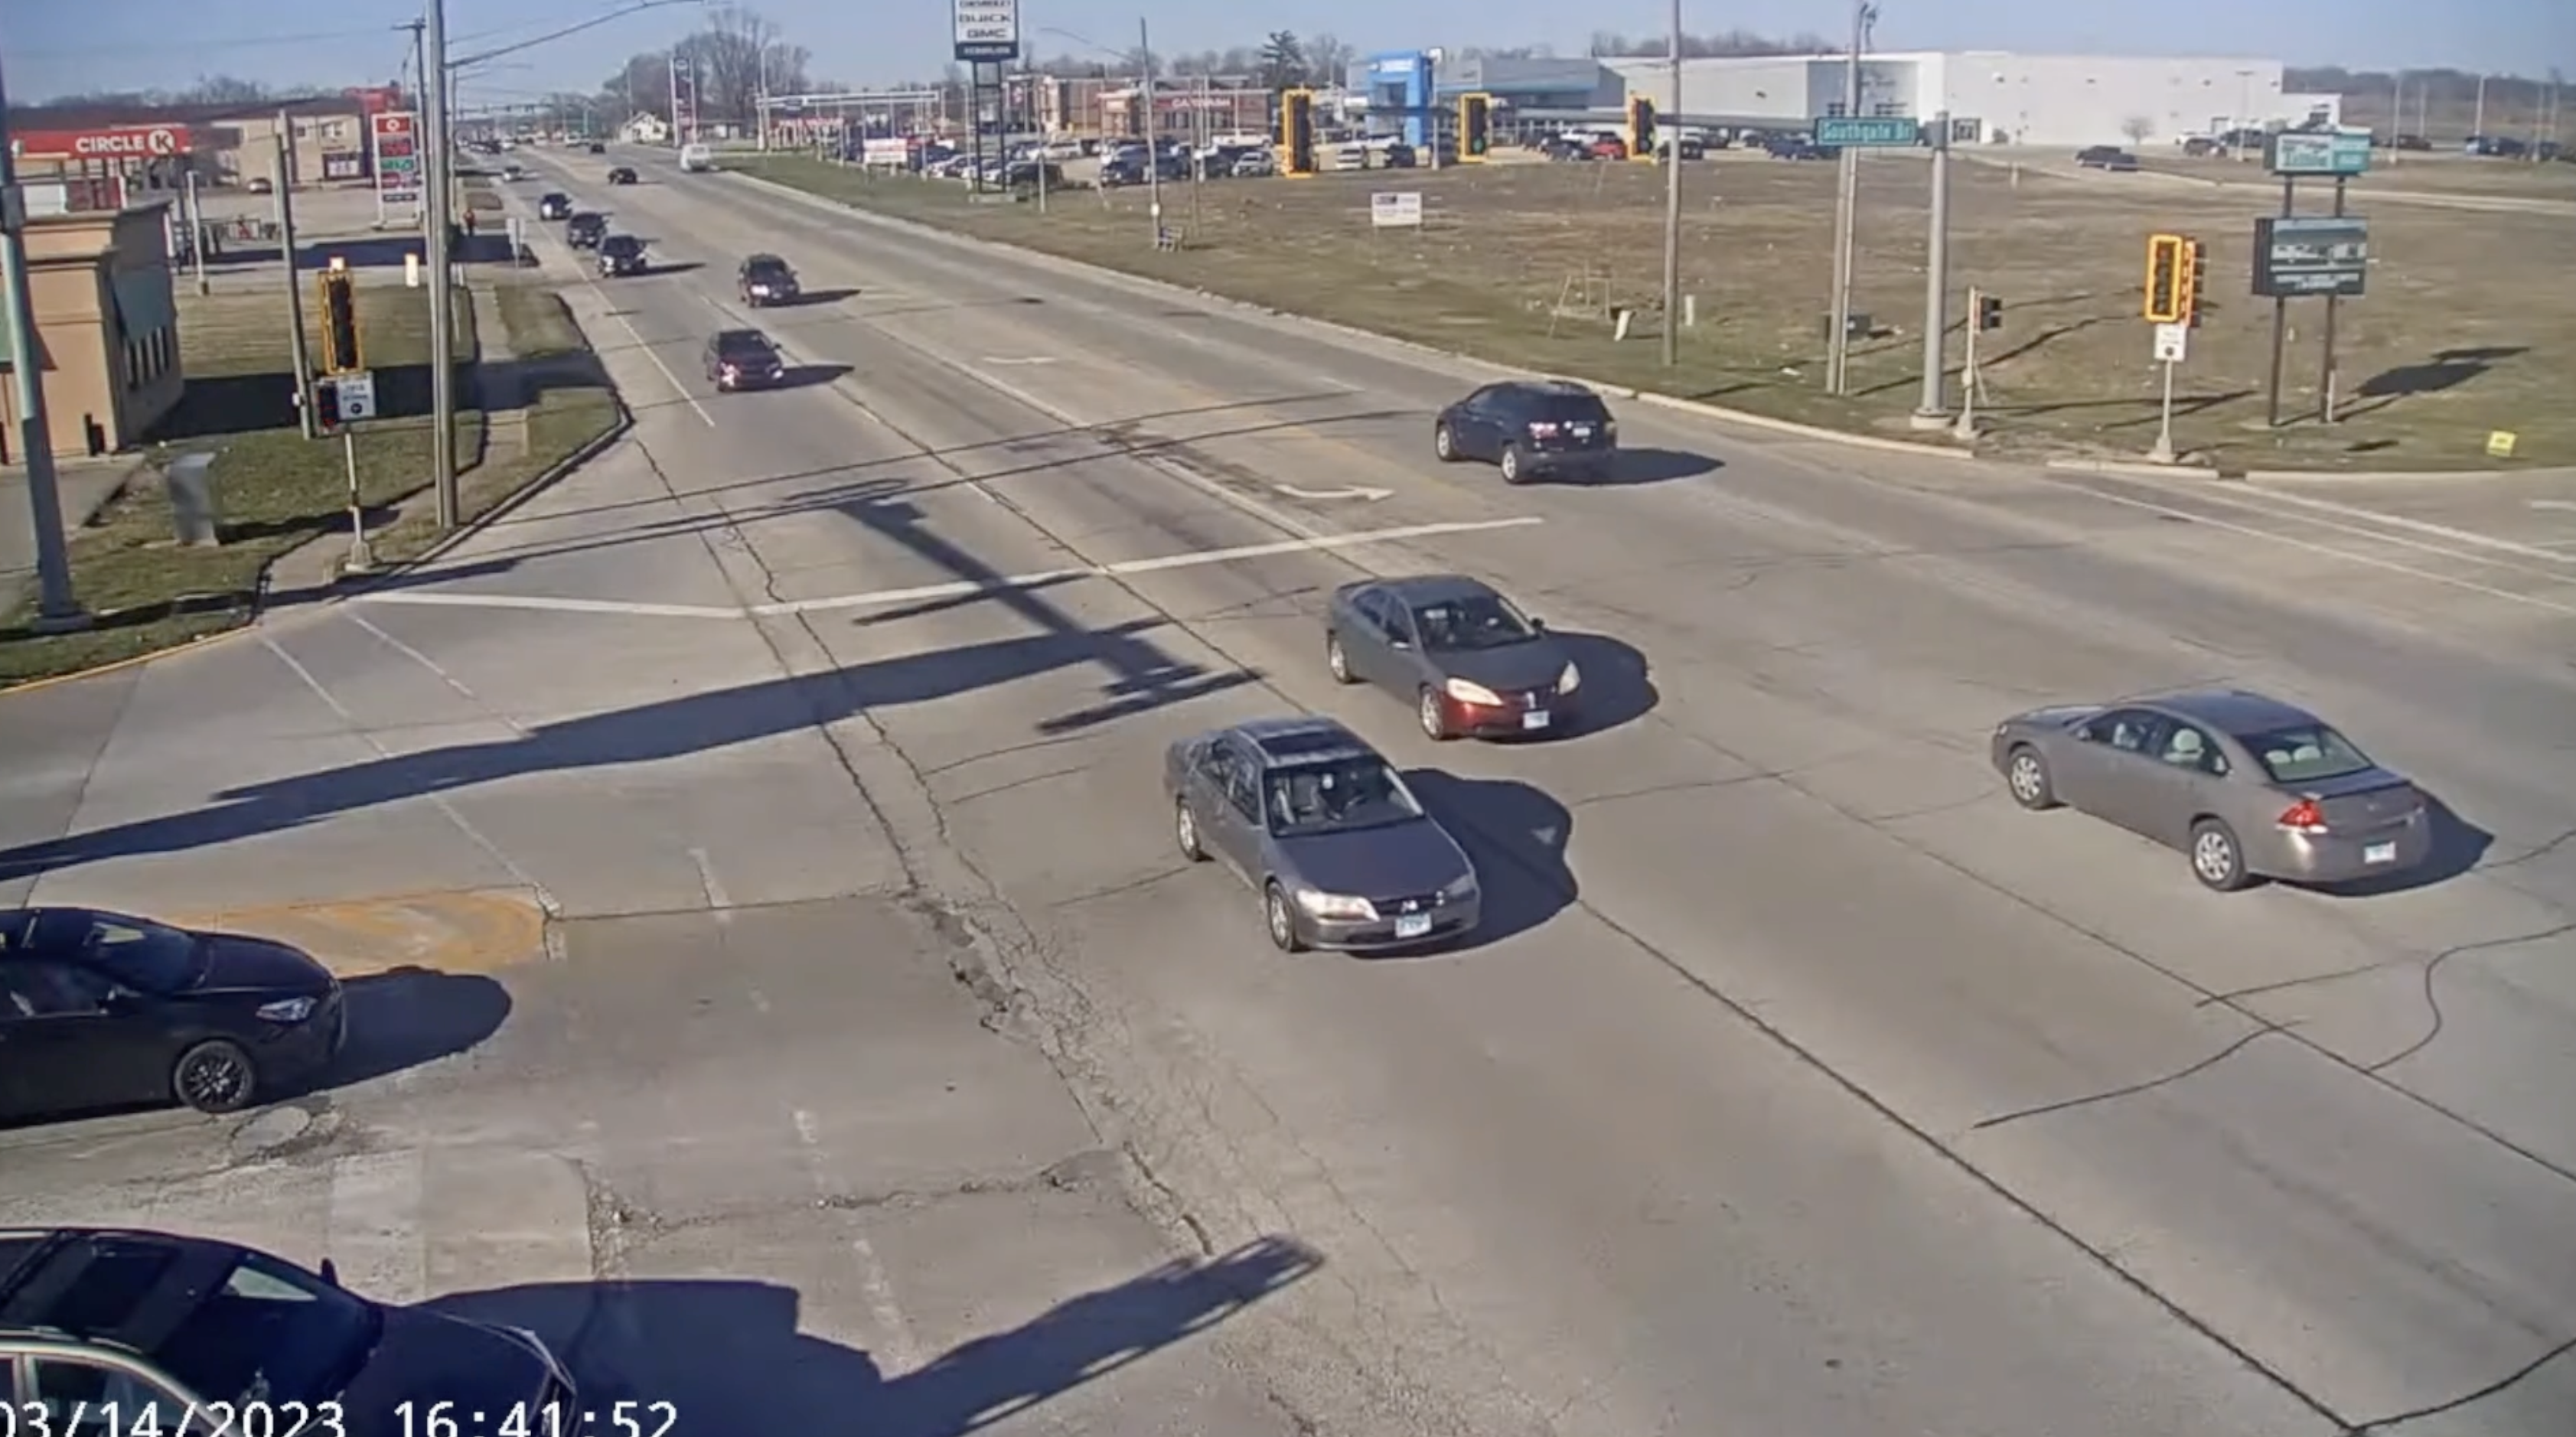
\includegraphics[width=\linewidth]{./Images/scene1.png}
    \caption{Scene 1: An intersection with a broader spectrum of car sizes.}
    \label{fig:scene1}
    \end{minipage}
    \hfill
    \begin{minipage}{0.45\textwidth}
    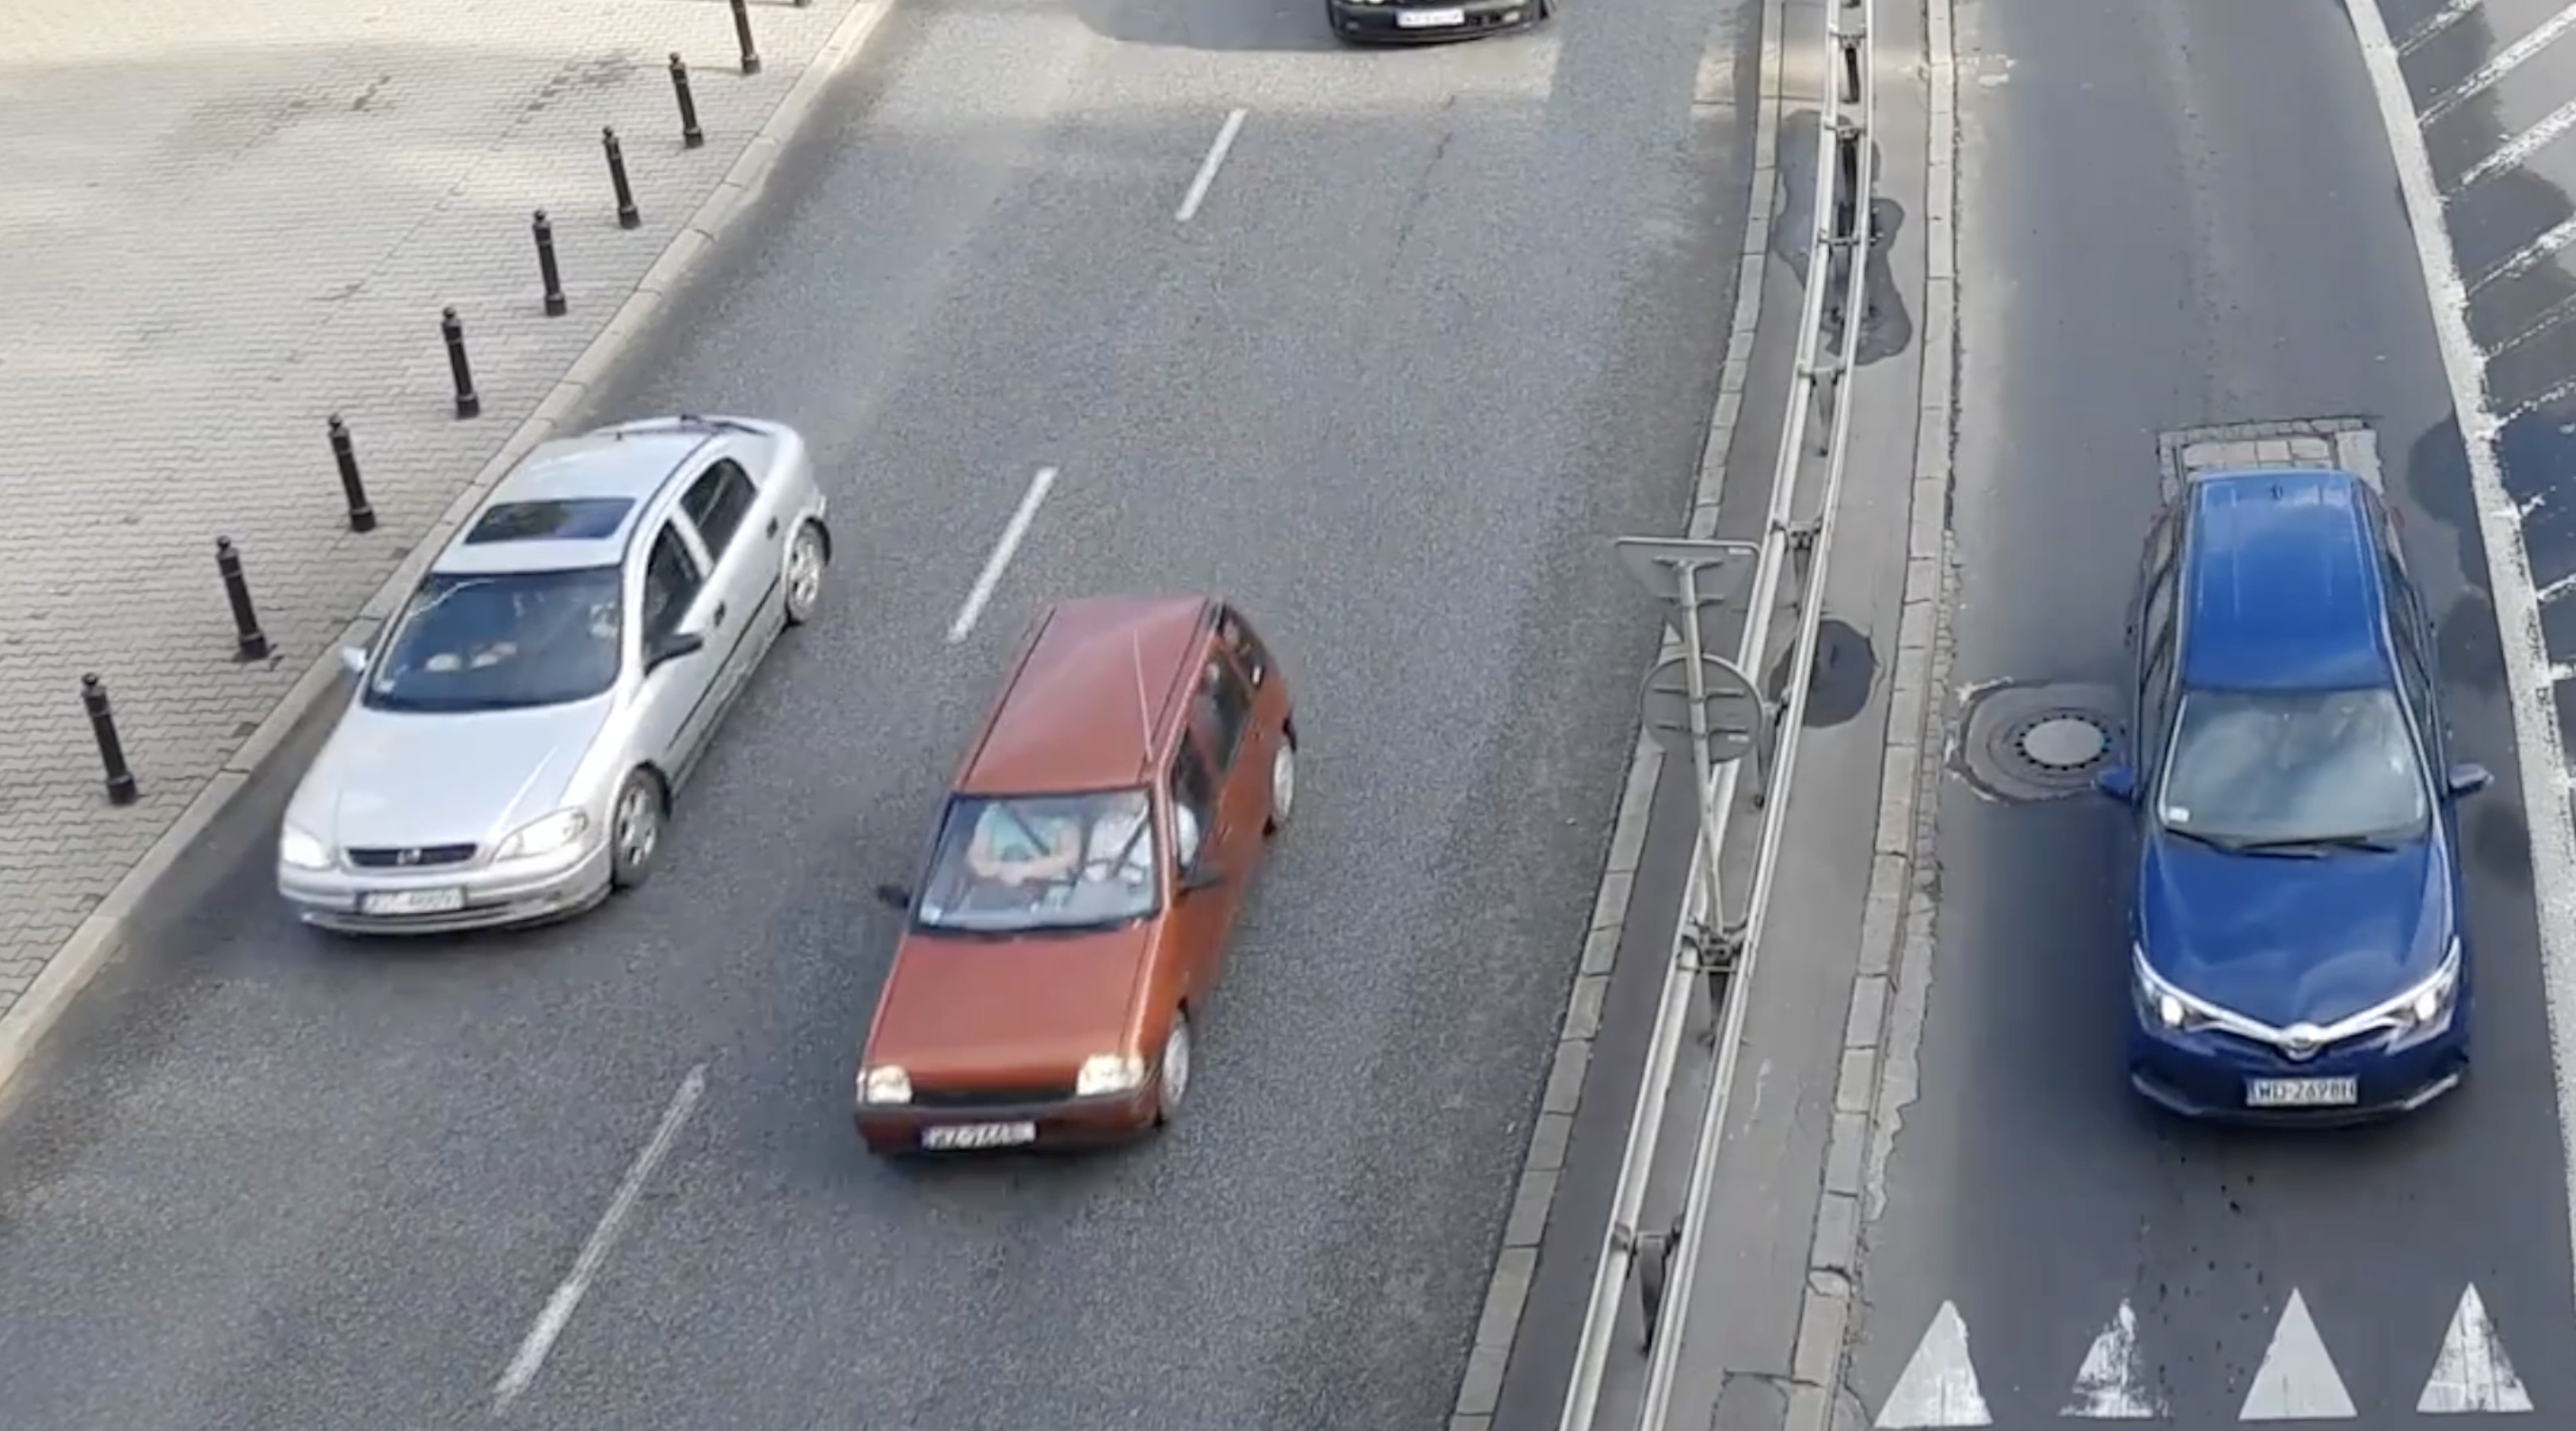
\includegraphics[width=\linewidth]{./Images/scene2.png}
    \caption{Scene 2: An overpass highway camera focused on larger vehicles given its location.}
    \label{fig:scene2}
    \end{minipage}
    \end{figure}
    

The visual comparison in Figures~\ref{fig:scene1} and~\ref{fig:scene2} illustrates the distinctive characteristics of each scene.

\begin{figure}[ht]
\centering
\includegraphics[width=\linewidth]{./Images/vari-viod.png}
\caption{Comparative graph showing gate activation across different scenes. This visualization underscores how specific channels are influenced by scene characteristics, reflecting the dynamic nature of gate behavior.}
\label{fig:comparative_analysis}
\end{figure}

The graph in Figure~\ref{fig:comparative_analysis} illustrates the variance in gate activation patterns when exposed to distinct scene attributes. The findings reveal a correlation between scene elements and the activation or suppression of particular channels, emphasizing the model's adaptability and sensitivity to contextual nuances.

\section{Discussion}
\label{sec:discussion}
Our study has successfully demonstrated that Gated Scene-Specific YOLO significantly enhances computational efficiency in environments with consistent features, such as stationary surveillance systems and traffic monitoring cameras. By focusing on fixed settings, the model's selective gating mechanism strategically deactivates irrelevant filters, reducing computational overhead. This approach aligns with the growing need for resource-efficient models in embedded systems and edge devices, where consistent environmental conditions prevail. While the model shows less adaptability to new or changing scenes, its performance in familiar settings suggests a substantial reduction in resource consumption without sacrificing accuracy. This characteristic makes it particularly valuable in applications where computational resources are limited, and operational consistency is guaranteed. Future work could focus on refining the gating mechanism to ensure minimal performance degradation over time and exploring similar efficiency-oriented approaches in other fixed-setting applications.

\section{Conclusion}
\label{sec:conclusion}
In this paper, we introduced the Gated Scene-Specific YOLO, a novel adaptation of the YOLO architecture that incorporates a dynamic gating mechanism to improve efficiency in fixed-setting object detection tasks. Our approach represents a significant stride towards resource-efficient deep learning, particularly for applications operating under consistent environmental conditions. The substantial computational savings achieved, along with the maintained accuracy, underscore the potential of selective gating in enhancing the performance of object detection models. While our model is tailored for fixed settings, its underlying principles may inspire broader research into resource optimization in various deep learning applications. As the demand for intelligent systems in resource-constrained environments grows, approaches like Gated Scene-Specific YOLO will be crucial in paving the way for more sustainable and efficient solutions.

\bibliographystyle{splncs04}
\bibliography{refs.bib}

\end{document}